\documentclass[a4paper,11pt]{jsarticle}


% 数式
\usepackage{amsmath,amsfonts}
\usepackage{amssymb}
\usepackage{bm}
% 画像
\usepackage[dvipdfmx]{graphicx}
\usepackage{here}
\usepackage{wrapfig}
\usepackage{listings,jvlisting}
\lstset{
  basicstyle={\ttfamily},
  identifierstyle={\small},
  commentstyle={\smallitshape},
  keywordstyle={\small\bfseries},
  ndkeywordstyle={\small},
  stringstyle={\small\ttfamily},
  frame={tb},
  breaklines=true,
  columns=[l]{fullflexible},
  numbers=left,
  xrightmargin=0zw,
  xleftmargin=3zw,
  numberstyle={\scriptsize},
  stepnumber=1,
  numbersep=1zw,
  lineskip=-0.5ex
}

\begin{document}

\title{画像実験課題A, B}
\author{1029323422 天野岳洋}
\date{\today}
\maketitle
\clearpage

\section{概要}
本レポートでは発展課題Aについて取り組んだ内容について述べたのちに, コンテストに対して
取り組んだ内容を述べる. そして最後に発展課題Bで取り組んだ内容について
説明を行う.
\section{AdvancedA}
発展課題Aの実装について述べる. 実装が簡単であったり,
定義通りにしか実装していない場合は説明は省略もしくは非常に簡単に述べるものとする.
また, 以後明記はしないが, 伝播層では(B, ?, 1)という形で伝播
するものとし, 逆伝播層では畳み込み層, プーリング層を除き(?, B)という形でデータを
扱っていることに注意したい.
\subsection{A1}
活性化関数としてSigmoid関数の代わりにRELU関数を用いるという内容である.
RELU関数は次のように表せる関数である.
\begin{equation}
  RELU(x)=
  \begin{cases}
    x & \text{if $x \geqq 0$} \\
    0 & \text{if $x < 0$}
  \end{cases}
\end{equation}
また逆伝播は以下のようである
\begin{equation}
  RELU'(x) =
  \begin{cases}
    1 & \text{if $x \geqq 0$} \\
    0 & \text{if $x < 0$}
  \end{cases}
\end{equation}
自分の実装を示す.
\begin{lstlisting}[caption=RELU]
  def __init__(self):
    pass

  def prop(self, x):
    self.input = x
    self.B, self.M, _ = x.shape
    return np.where(x <= 0, 0, x)
    
  def back(self, delta):
    return delta * (np.where(self.input <= 0, 0, 1).reshape(self.B, self.M).T)
\end{lstlisting}

np.whereにより, 0以下を0にしてそれ以外をxのままにしている.
逆伝播層では, xにする代わりに1にしている. ここで, 行列の形が違うことに注意して変形を行っている.

\subsection{A2}
Dropout層を実装せよという内容である. Dropout層の定義は以下のものである.
\begin{equation}
  Dropout(x) =
  \begin{cases}
    x & \text{(ノードが無視されない場合)} \\
    0 & \text{(ノードが無視される場合)}
  \end{cases}
\end{equation}
また逆伝播では,
\begin{equation}
  \begin{split}
    \frac{\partial En}{\partial x} = & \frac{\partial En}{\partial y}\frac{\partial y}{\partial x}  \\= &
    \begin{cases}
      \frac{\partial En}{\partial y} & \text{(ノードが無視されない場合)} \\
      0                              & \text{(ノードが無視された場合)}
    \end{cases}
  \end{split}
\end{equation}
具体的な実装の説明に移る.Dropout層のハイパーパラメータを$\rho$とする.
このハイパーパラメータをもとにマスクされるノードの個数を定める.
その後random.choiceによってどのノードがマスクされるかを選択し,
適切な処理をすればよい. またテストの際には定義にのっとり,
マスクはせずに定数倍を行っている.
\begin{lstlisting}[caption=Dropout]
  def __init__(self, phi, M):
    self.phi = phi
    self.msk_num = int(M*phi)
    self.M = M

  def prop(self, x):
    B = x.shape[0]
    M = self.M
    drop_random = np.repeat(np.random.choice(M, self.msk_num), B).reshape(-1, B).T
    mask_vector = np.ones((B, M))
    mask_vector[np.repeat(np.arange(B), self.msk_num), drop_random.flatten()] = 0
    self.msk = mask_vector.reshape(B, -1, 1)
    return x * self.msk

  def back(self, delta):
    return delta * self.msk.reshape(self.B, self.M).transpose(1, 0)

  def test(self, x):
    return x * (1 - self.phi)
\end{lstlisting}
prop層のmask\_vectorの作り方が少し複雑なので, 例を挙げて説明する.
例えば, msk\_num = 3, M = 5, B = 2の時を考える. 今drop\_randomは
0$\sim$4から3個重複を許さずに選び, それを2回ずつ繰り返し, 次元を(3, 2)に変え転置をとるものだから, 順番に追っていくと,
例えば, 0, 1, 3が選ばれたとすると, 次のような形で処理が行われ, drop\_randomが得られることとなる.

$$
  [0, 1, 3] \rightarrow [0, 0, 1, 1, 3, 3] \rightarrow
  \begin{bmatrix}
    0 & 0 \\
    1 & 1 \\
    3 & 3 \\
  \end{bmatrix}
  \rightarrow \begin{bmatrix}
    0 & 1 & 3 \\
    0 & 1 & 3 \\
  \end{bmatrix}
$$
続いて同様にmask\_vectorの推移を説明する. まず, (B, M)の形で全て1
が入ったもので初期化され, その後mask\_vector[[0,0,0,1,1,1][0 1 3 0 1 3]] = 0
となっている. つまり

$$
  mask\_vector \rightarrow \begin{bmatrix}
    1 & 1 & 1 & 1 & 1 \\
    1 & 1 & 1 & 1 & 1
  \end{bmatrix} \rightarrow
  \begin{bmatrix}
    0 & 0 & 1 & 0 & 1 \\
    0 & 0 & 1 & 0 & 1
  \end{bmatrix}
$$
というような推移になっている. あとはこれを適切な形に変形させ,
入力データとアダマール積をとればある特定のノードの出力が0になっていることが
簡単にわかる. また逆伝播層でも入力のshapeが違うことを除けば同様に
アダマール積をとるだけである.
\subsection{A3}
Batch-Normalizationを行えというものである.
Batch normalization層は、ニューラルネットワークの学習において、過学習を防止し、学習速度を上げるために使用される。特に、深いニューラルネットワークでは、層を重ねることで、入力データのパラメータの分布が変化しやすくなり、学習が容易に進まない問題が生じる。これを解消するために、batch normalization層は、入力データを正規化することで、学習を安定させる効果がある。

具体的に、batch normalization層では、各ミニバッチの入力データの平均値と標準偏差を計算し、それらを使って入力データを正規化する。また、batch normalization層はデータの分布が異なることを考えて, 学習時と推論時で別々に平均や標準偏差を計算する。
定義式は次のように表せる.
\begin{align*}
  \mu_B      & = \frac{1}{B}\sum_{i=1}^{B} x_i                    \\
  \sigma_B^2 & = \frac{1}{B}\sum_{i=1}^{B} (x_i - \mu_B)^2        \\
  \hat{x_i}  & = \frac{x_i - \mu_B}{\sqrt{\sigma_B^2 + \epsilon}} \\
  y_i        & = \gamma\hat{x_i} + \beta
\end{align*}
さらに逆伝播を導出する. $\frac{\partial L}{\partial y_i}$は与えられていることに注意する.
\begin{align*}
   & \frac{\partial L}{\partial \hat{x_i}} = \gamma\frac{\partial L}{\partial y_i} &
   & \frac{\partial L}{\partial \gamma} = \frac{\partial L}{\partial y_i}\hat{x_i} &
   & \frac{\partial L}{\partial \beta} = \frac{\partial L}{\partial y_i}
\end{align*}
次に, $\hat{x_i}$について
\begin{align*}
   & \frac{\partial \hat{x_i}}{\partial (x_i -\mu_B)} = \frac{1}{\sqrt{\sigma_B^2 + \epsilon}}                        &
   & \frac{\partial \hat{x_i}}{\partial \sigma_B^2} = (x_i - \mu_B)\frac{-1}{2}(\sigma_B^2 + \epsilon)^{-\frac{3}{2}}
\end{align*}
さらに, $\sigma_B^2$について
\begin{align*}
  \frac{\partial \sigma_B^2}{\partial (x_i - \mu_B)} = \frac{2}{B} (x_i - \mu_B)
\end{align*}
また, 自明ではあるが, $x_i - \mu_B$について
\begin{align*}
  \frac{\partial (x_i - \mu_B)}{\partial x_i} = 1 &  &
  \frac{\partial (x_i - \mu_B)}{\partial \mu_B} = -1
\end{align*}
さらに, $\mu_B$について,
\begin{align*}
  \frac{\partial \mu_B}{\partial x_i} = \frac{1}{B}
\end{align*}
以上より次のようにかける.
\begin{align*}
  \frac{\partial L}{\partial x_k} & = \sum_{i=1}^{B}\frac{\partial L}{\partial y_i}\frac{\partial y_i}{\partial x_k}                                                                                                                                                                                                                                                                          \\
                                  & = \sum_{i=1}^{B}\frac{\partial L}{\partial y_i}\frac{\partial y_i}{\partial \hat{x_i}}\frac{\partial \hat{x_i}}{\partial x_k}                                                                                                                                                                                                                             \\
                                  & = \sum_{i=1}^{B}\sum_{l=1}^{B}\frac{\partial L}{\partial y_i}\gamma(\frac{\partial \hat{x_i}}{\partial (x_l - \mu_B)} + \frac{\partial \hat{x_i}}{\partial \sigma_B^2}\frac{\partial \sigma_B^2}{\partial (x_l - \mu_B)})(\frac{\partial (x_l - \mu_B)}{\partial x_k} + \frac{\partial (x_l - \mu_B)}{\partial \mu_B}\frac{\partial \mu_B}{\partial x_k}) \\
                                  & = \sum_{i=1}^{B}\frac{\partial L}{\partial y_i}\gamma(\frac{\partial \hat{x_i}}{\partial (x_k - \mu_B)} +\frac{\partial \hat{x_i}}{\partial \sigma_B^2}\frac{\partial \sigma_B^2}{\partial (x_k - \mu_B)})                                                                                                                                                \\ & \qquad - \frac{1}{B}\sum_{i=1}^{B}\sum_{l=1}^{B}\frac{\partial L}{\partial y_i}\gamma(\frac{\partial \hat{x_i}}{\partial (x_l - \mu_B)} + \frac{\partial \hat{x_i}}{\partial \sigma_B^2}\frac{\partial \sigma_B^2}{\partial (x_l - \mu_B)})\\
                                  & = \sum_{i=1}^{B}\frac{\partial L}{\partial y_i}\gamma(\frac{\partial \hat{x_i}}{\partial (x_k - \mu_B)} +\frac{\partial \hat{x_i}}{\partial \sigma_B^2}\frac{\partial \sigma_B^2}{\partial (x_k - \mu_B)})                                                                                                                                                \\ & \qquad - \frac{1}{B}\sum_{i=1}^{B}\frac{\partial L}{\partial y_i}\gamma(\frac{\partial \hat{x_i}}{\partial (x_i - \mu_B)})  \\ &  \qquad\qquad - \frac{1}{B} \sum_{i=1}^{B}\frac{\partial \hat{x_i}}{\partial \sigma_B^2}\sum_{l=1}^{B}\frac{\partial \sigma_B^2}{\partial (x_l - \mu_B)} \\
                                  & = \frac{\partial L}{\partial y_k}\gamma\frac{\partial \hat{x_k}}{\partial (x_k - \mu_B)} + \sum_{i=1}^{B}\frac{\partial L}{\partial y_i}\gamma\frac{\partial \hat{x_i}}{\partial \sigma_B^2}\frac{\partial \sigma_B^2}{\partial (x_k - \mu_B)}                                                                                                            \\ & \qquad - \frac{1}{B}\sum_{i=1}^{B}\frac{\partial L}{\partial y_i}\gamma(\frac{\partial \hat{x_i}}{\partial (x_i - \mu_B)})
  - \frac{1}{B}\sum_{i=1}^{B}\frac{\partial \hat{x_i}}{\partial \sigma_B^2}\sum_{l=1}^{B}\frac{\partial \sigma_B^2}{\partial (x_l - \mu_B)}
\end{align*}

逆伝播は以上式によって求められる.
教科書との対応だが, \footnote{教科書iをここではkとしています.}
\begin{align*}
   & \frac{\partial E_n}{\partial \hat{x_k}} \cdot \frac{1}{\sqrt{\sigma_B^2 + \epsilon}} &  & = \frac{\partial L}{\partial y_k}\gamma\frac{\partial \hat{x_k}}{\partial (x_k - \mu_B)} \\
   & \frac{\partial E_n}{\partial \sigma_B^2} \cdot \frac{2(x_k - \mu_B)}{B}              &  & =
  \sum_{i=1}^{B}\frac{\partial L}{\partial y_i}\gamma\frac{\partial \hat{x_i}}{\partial \sigma_B^2}\frac{\partial \sigma_B^2}{\partial (x_k - \mu_B)}                                   \\
   & \frac{\partial E_n}{\partial \mu_B} \cdot \frac{1}{B}                                &  & =
  - \frac{1}{B}\left(
  \sum_{i=1}^{B}\frac{\partial L}{\partial y_i}\gamma(\frac{\partial \hat{x_i}}{\partial (x_i - \mu_B)})
  + \sum_{i=1}^{B}\frac{\partial \hat{x_i}}{\partial \sigma_B^2}\sum_{l=1}^{B}\frac{\partial \sigma_B^2}{\partial (x_l - \mu_B)}
  \right)
\end{align*}
したがって実装は以下のようになる.
\begin{lstlisting}[caption=Batch-Normalization-prop]
  def prop(self, x):
    #x = B * M * 1
    self.x = x
    self.B, self.M, _ = x.shape
    self.microB = np.sum(x, axis=0) / x.shape[0]
    self.sigmaB = np.sum((x - self.microB) ** 2, axis=0) / x.shape[0]
    self.normalize_x = (x - self.microB) / np.sqrt(self.sigmaB + BatchNormalize.eps)
    self.y = self.ganma * self.normalize_x + self.beta
    # yをreturn
    return self.y
\end{lstlisting}

\begin{lstlisting}[caption=Batch-Normalization-back]
  def back(self, delta):
    delta_xi_head = delta * self.ganma
    delta_sigmaB2 = np.sum(delta_xi_head * (self.x.reshape(self.B, self.M).T - self.microB) * (-1/2) * np.power(self.sigmaB + BatchNormalize.eps, -3/2), axis=1).reshape(self.M, 1)
    delta_microB = np.sum(delta_xi_head * (-1 / np.power(self.sigmaB + BatchNormalize.eps, 1/2)), axis=1).reshape(self.M, 1) + (-2) * delta_sigmaB2 * np.sum(self.x.reshape(self.B, self.M).T - self.microB, axis=1).reshape(self.M, 1)
    delta_a = delta_xi_head * np.power(self.sigmaB + BatchNormalize.eps, -1/2) + delta_sigmaB2 * 2 * (self.x.reshape(self.B, self.M).T - self.microB) / self.B + delta_microB / self.B
    delta_ganma = np.sum(delta * self.normalize_x.reshape(self.B, self.M).T, axis=1).reshape(self.M, 1)
    delta_beta = np.sum(delta, axis=1).reshape(self.M, 1)
\end{lstlisting}

\subsection{A4}
様々な最適化手法を試すものとなっている. 実際の実装は以下のようである.
\begin{lstlisting}
  def adagrad(self, w_b, delta, h):
    h = h + delta * delta
    return w_b - Batch.my * np.power(h, -1/2) * delta, h

  def RMSProp(self, w_b, delta, h):
    h = Batch.rho * h + (1 - Batch.rho) * delta * delta
    return w_b - Batch.my * (1 / (np.power(h, 1/2) + Batch.eps) ) * delta, h

  def AdaDelta(self, w_b, delta, h, s):
    h = Batch.rho * h + (1 - Batch.rho) * delta * delta
    delta_w = - np.power(s + Batch.eps, 1/2) * np.power(h + Batch.eps, -1/2) * delta
    s = Batch.rho * s + (1 - Batch.rho) * delta * delta
    w = w_b + delta_w
    return w, h, s

  def Adam(self, w_b, delta, t, m, v):
    t = t + 1
    m = Batch.beta1 * m  + ( 1 - Batch.beta1 ) * delta
    v = Batch.beta2 * v  + ( 1 - Batch.beta2 ) * delta * delta
    m_head = m / ( 1 - np.power(Batch.beta1, t))
    v_head = v / ( 1 - np.power(Batch.beta2, t))
    W = w_b - Batch.alpha_para * m_head / (np.power(v_head, 1/2) + Batch.eps)
    return W, m, v, t
\end{lstlisting}
実装の方法は省略するものとし, それぞれの学習方法がどのようなものであるかを考察する.

\subsubsection*{Momentum付きSGD}
SGDでは振動してしまい収束しないという状況が考えられる.
Momentum付きSGDでは現在の勾配だけでなく, 過去の差分を用いることによって,
この振動を抑えている.

例えば$ y = x^2 $のグラフにおいて今の地点が$x = 1$であり, 学習率が1であった場合,
次の地点は$x = -1$となりさらにその次は$x = 1$となり振動してしまう.
一方で, Momentum付きSGDにすることによって, 解消される. 例えば, 0.9だけ過去の差分を取り入れるとしたら,
$x = 1$の次は, $x = - 1$でありさらにその次は, $\Delta = 0.9 * -2 + 1 * 2 = 0.2$であるので, $x = -1 + 0.2 = -0.8$...となり
振動が抑えられていることがわかる.
\subsubsection*{AdaGrad}
学習率を調節するものである. SGDの問題として, 収束速度が各軸によってまばらで
あるという問題がある. 具体的に言うと, ある軸で見たときに勾配が緩やかな状況を考えると,
その軸での更新幅は小さく, それ以外の軸での更新幅は大きいということが起こる. すなわち, 学習を進めた際に
それ以外の軸では収束しているのに, その軸が収束していないという状況が考えられる.
これを解消するために, 更新が少ない軸では更新幅を大きくするという学習率の面での工夫がAdaGradである.
教科書のhは今までの更新の2乗の総和であり, hが大きい場所程更新幅は小さい。またその逆もしかりである.
\subsubsection*{RMSProp}
AdaGradでは一度大きな更新が行われた軸では学習率が大きく下がってしまったままという問題が発生した.
その問題を解決するために, hを今までの単なる総和ではなく, 等比数列的に過去の更新幅を減衰していって加えていくという
変更を加えたものである. またこのような処理を加えることによって, hが0に収束してしまう場合が考えられるので,
0割りを防ぐために$\epsilon$が分母に加えられている.
\subsubsection*{Adadelta}
RMSProp以下では, $\Delta w$の次元が$w$とマッチしていないという事態になっていた.
実際, $\Delta w$は基本的に勾配の定数倍であったので, その次元はwの次元を$Dimw$とすると,
$1/Dimw$となる.
これは微分が損失関数の変位(定数)をwで割ったものの微小極限であることを考えれば明らかである.
よって$w + \Delta w$は次元が違う二つの値を足していることとなる.
そのため, なにか不都合な問題が起こった(何が問題なのかを調べきることができませんでした.)
これを解決するのがAdadeltaである. 実際に次元を見てみると,
hの次元は $1 / Dimw^2$であり, $s$の次元を$Dimw^2$とすると, $\Delta w$の次元は
$Dimw * Dimw / Dimw = Dimw$となり, うまくいっている.\footnote{$s$の次元を知るのに, $\Delta w$の次元が必要で,
  その逆も成り立つので, 一度仮定が必要になっています. うまく示せていませんね...}
\subsubsection*{Adam}
Momentum + RMSPropである. これは式を見えれば簡単に理解できる.
(54), (55)の補正について説明する.
(54)の説明だけで十分である. 簡易的に一次元値であることを仮定し, さらに$\beta_1$
を$\beta $としている. 教科書式(52)を変形していく.
$\frac{\delta E_n}{\delta W}$ をgとする.
\begin{align*}
  m_t = & (1 - \beta)g_t + \beta m_{t-1}                                \\
  =     & (1 - \beta)g_t + \beta (1 - \beta)(g_{t-1}) + \beta^2 m_{t-2} \\
  =     & \dots                                                         \\
  =     & (1 - \beta)\sum_{i=1}^{t}\beta^{t-i}g_i + \beta^{t}m_{0}
\end{align*}
ここで$g_t$と$m_t$の平均についての関係性を調べると
\begin{align*}
  \mathbb{E}\lbrack m_t \rbrack = & \mathbb{E}\lbrack (1 - \beta)\sum_{i=1}^{t}\beta^{t-i}g_i + \beta^{t}m_{0} \rbrack                     \\
  =                               & (1-\beta)\sum_{i=1}^{t}\beta^{t-i}\mathbb{E}\lbrack g_i \rbrack + \beta^t\mathbb{E}\lbrack m_0 \rbrack \\
  =                               & (1 - \beta)\mathbb{E}[g_t]\frac{1-\beta^t}{1-\beta}                                                    \\
  =                               & (1 - \beta^t)\mathbb{E}[g_t]
\end{align*}
よって不偏性を保つために, 式(54)によって補正していることが分かった.\footnote{そもそもなぜ不偏性が必要なのかがわからなかった.時間とともに, mtの値が大きくなっていくのが問題?}

\subsubsection*{学習速度の比較}
次に以上6パターンでの学習速度の比較を行う.
下図左は訓練データに対する, 下図右は
テストデータに対するクロスエントロピー誤差を表している.
なお最適化に関するハイパーパラメータは教科書にて推奨されているものを使った.
\begin{figure}[H]
  \begin{minipage}[b]{0.45\linewidth}
    \centering
    \includegraphics*[keepaspectratio, width=0.9\linewidth]{loss_history.png}
    \caption{train\_loss}
  \end{minipage}
  \begin{minipage}[b]{0.45\linewidth}
    \centering
    \includegraphics*[keepaspectratio, width=0.9\linewidth]{val_loss_history.png}
    \caption{validation\_loss}
  \end{minipage}

  これを踏まえると, 現在のモデルに対しては, 訓練データ, テストデータともにmomentum付きSGDが
  もっともよい学習方法であると結論付けることが出来た.

\end{figure}
\subsection{A6}
畳み込み層の実装を行う.
以下の手順で畳み込み層の実装を行った.
\begin{enumerate}
  \item 畳み込みフィルタを定義する。初期化は今回正規分布に従う値にした.
  \item 入力データを畳み込みフィルタを適用するために、フィルタサイズに合わせて切り分ける。
  \item それぞれの切り分けられた部分に対して畳み込みフィルタを適用し、その結果を適切に並べたものを出力とする。
  \item バイアスを加える.
\end{enumerate}
特に, 2.が非常にややこしいのでこの部分を説明する.
\subsubsection*{切り分け}
切り分けであるが, 今回は畳み込み前後でサイズが変わらないほうが嬉しいため,
フィルタサイズは奇数長であるという制限を設けている.さらにこの切り分けの前に, paddingを行っている.
paddingはnumpy.padで簡単に実装できる.
まずは切り分けを行うコードを提示する.
\begin{lstlisting}[caption=x2X]
  def x2X(self, x, R):
    B, ch, x_length, x_width = x.shape
    dx = x_length - R + 1
    dy = x_width - R + 1
    altx = np.zeros((B, ch, R, R, dx, dy))
    for i in range(R):
        for j in range(R):
            altx[:, :, i, j, :, :] = x[:, :, i:i+dx, j:j+dy]
    return altx.transpose(1, 2, 3, 0, 4, 5).reshape(R*R*ch, dx*dy*B)
\end{lstlisting}

順に説明を行う. xは切り分けを行う前のテンソルであり, Rはフィルタサイズになっている.
ここでまず, xのシェイプから各種値を取得している. 次から具体的な切り分けの作業を行っていくが,
まずfor文を使う回数をなるべく少なくするために, 大きな四角形でくりぬくことで, 切り分け後の一行一列目の値だけを並べたものを
取得できる. このようにすることで繰り返し数をフィルタサイズ * フィルタサイズ程度に収めることができる.
図を使って説明を行う. 以下の図はB = 1, ch = 1 であることに注意したい.
\begin{figure}[H]
  \centering
  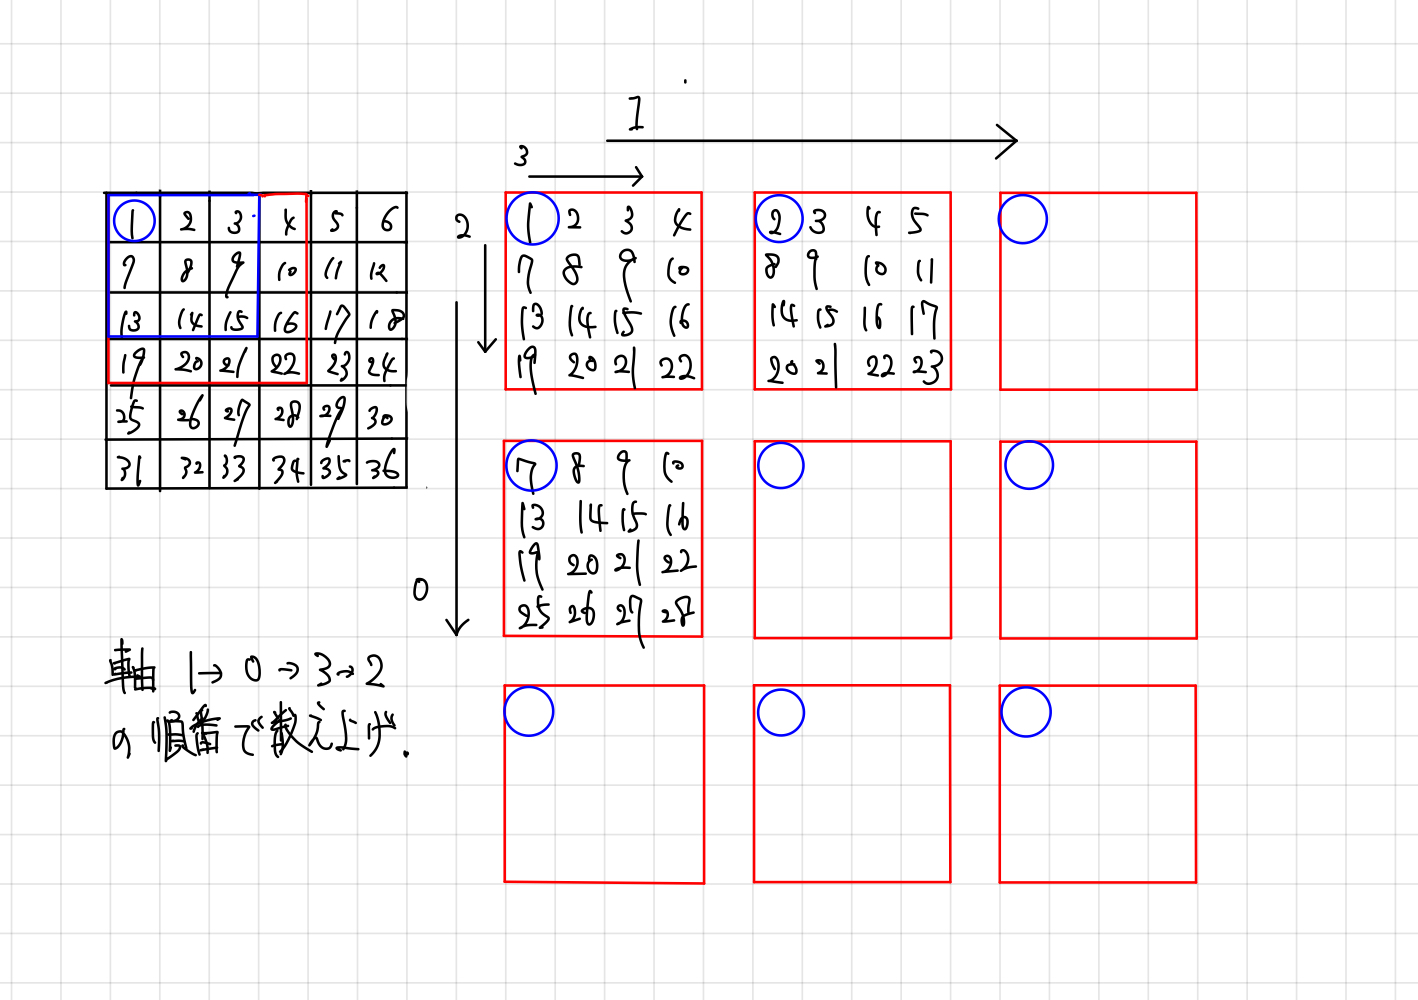
\includegraphics[height = 7cm]{rep_conv.jpg}
  \caption{x2X}
\end{figure}
赤四角の大きさがdx, dyである. 左の大きなテンソルの初期化を次に行っている.
その次のfor文内でそのテンソルにくりぬいている.
最後のtransposeが数え上げの順番を変えている.その後にreshapeで適切な形にしている.

\subsubsection*{適用}
切り分けさえできれば後はたやすい. 順伝播は次のようなものになる.
\begin{lstlisting}[caption=convolution-prop]
  self.B = x.shape[0]
    r = self.R // 2
    self.r = r
    x_prime = np.pad(x, [(0,), (0, ), (r,), (r,)], "constant")
    self.X = self.x2X(x_prime, self.R)
    self.Y = np.dot(self.filter_W, self.X) + self.bias
    # self.Y -> K * (imgsize * B)
    self.Y = self.Y.reshape(self.K, self.B, self.imr, self.imr).transpose(1, 0, 2, 3)
    # self.Y -> B * K * imlen * imlen
    return self.Y
\end{lstlisting}

\subsubsection*{逆伝播}
教科書通りの実装である.
気をつけなければならない点として, x2Xの逆の作業を行う必要があることと,
paddingを行っているのでその部分を切り取ったものを出力しなければならないことがあるが,
それ以外は簡単である.
\begin{lstlisting}[caption=X2x]
  def X2x(self, X):
    w = self.R
    bigL = self.imr + self.r*2 - w + 1
    bigW = self.imr + self.r*2 - w + 1
    x = np.zeros((self.B, self.ch, self.imr + self.r * 2, self.imr + self.r * 2))
    arX = X.reshape(self.ch, w, w, self.B, bigL, bigW).transpose(3, 0, 1, 2, 4, 5)
    for i in range(w):
        for j in range(w):
            x[:, :, i:i+bigL, j:j+bigW] = arX[:, :, i, j, :, :]
    return x
\end{lstlisting}
\begin{lstlisting}[caption=convolution-back]
  def back(self, delta):
    #delta -> B * K * imlen * imlen
    delta = delta.transpose(1, 0, 2, 3).reshape(self.K, -1)
    #delta -> K * (B * imlen * imlen)
    delta_filter_x = np.matmul(self.filter_W.T, delta)
    delta_filter_W = np.matmul(delta, self.X.T)
    delta_filter_b = np.sum(delta, axis=0)
    self.filter_W = self.filAdam.update(delta_filter_W)
    self.bias = self.biAdam.update(delta_filter_b)
    return self.X2x(delta_filter_x)[:, :, self.r:self.r + self.imr, self.r:self.r + self.imr]
\end{lstlisting}

実際に十分に学習させたフィルタで畳み込みを行うと次のようになる.
\begin{figure}[H]
  \centering
  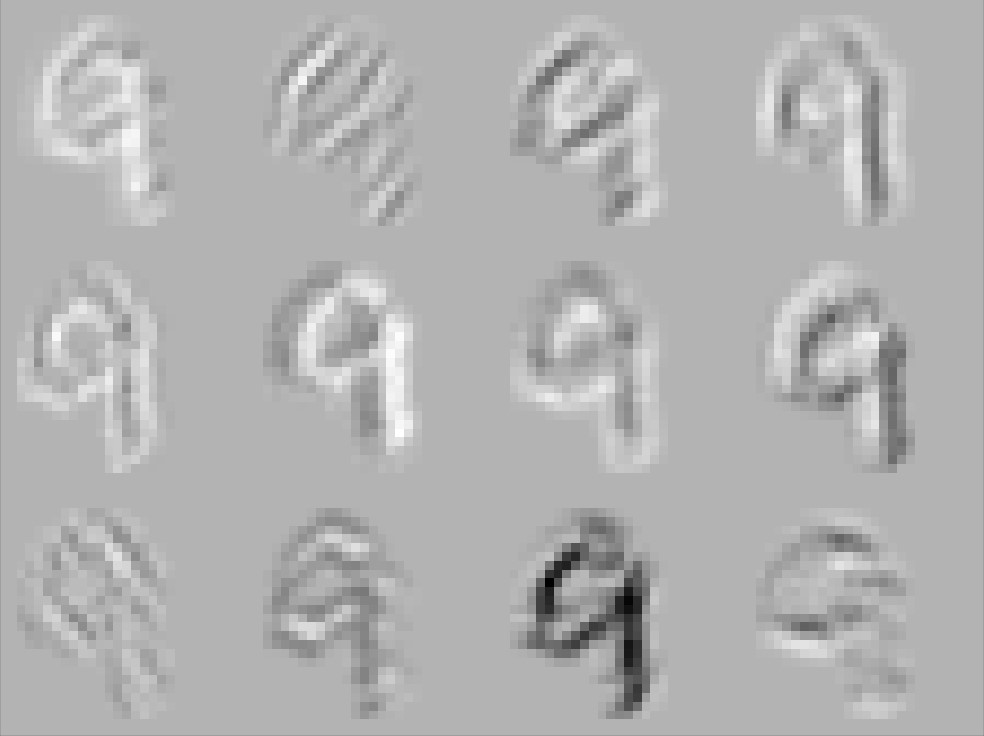
\includegraphics[height = 5cm]{conv.jpg}
  \caption{convolution}
\end{figure}


\subsection{A7}
プーリングを行う.今回はMaxPoolingを行うものとする.
以下の手順での実装とする.
\begin{enumerate}
  \item 切り分けを行い, その窓ごとの最大値とその位置を取得
  \item 適切な形に変形
  \item 取得した位置をもとに, 逆伝播してきた微分値を代入.
  \item x2Xの逆の作業によって適切な形に変形
\end{enumerate}

全て以前に出てきたものであるので実装は簡単であるが,
想像がつきづらいので, B = 1, ch = 1, の状況下で具体的に説明を行う.
まずは以下の図を見てもらいたい.

\begin{figure}[h]
  \centering
  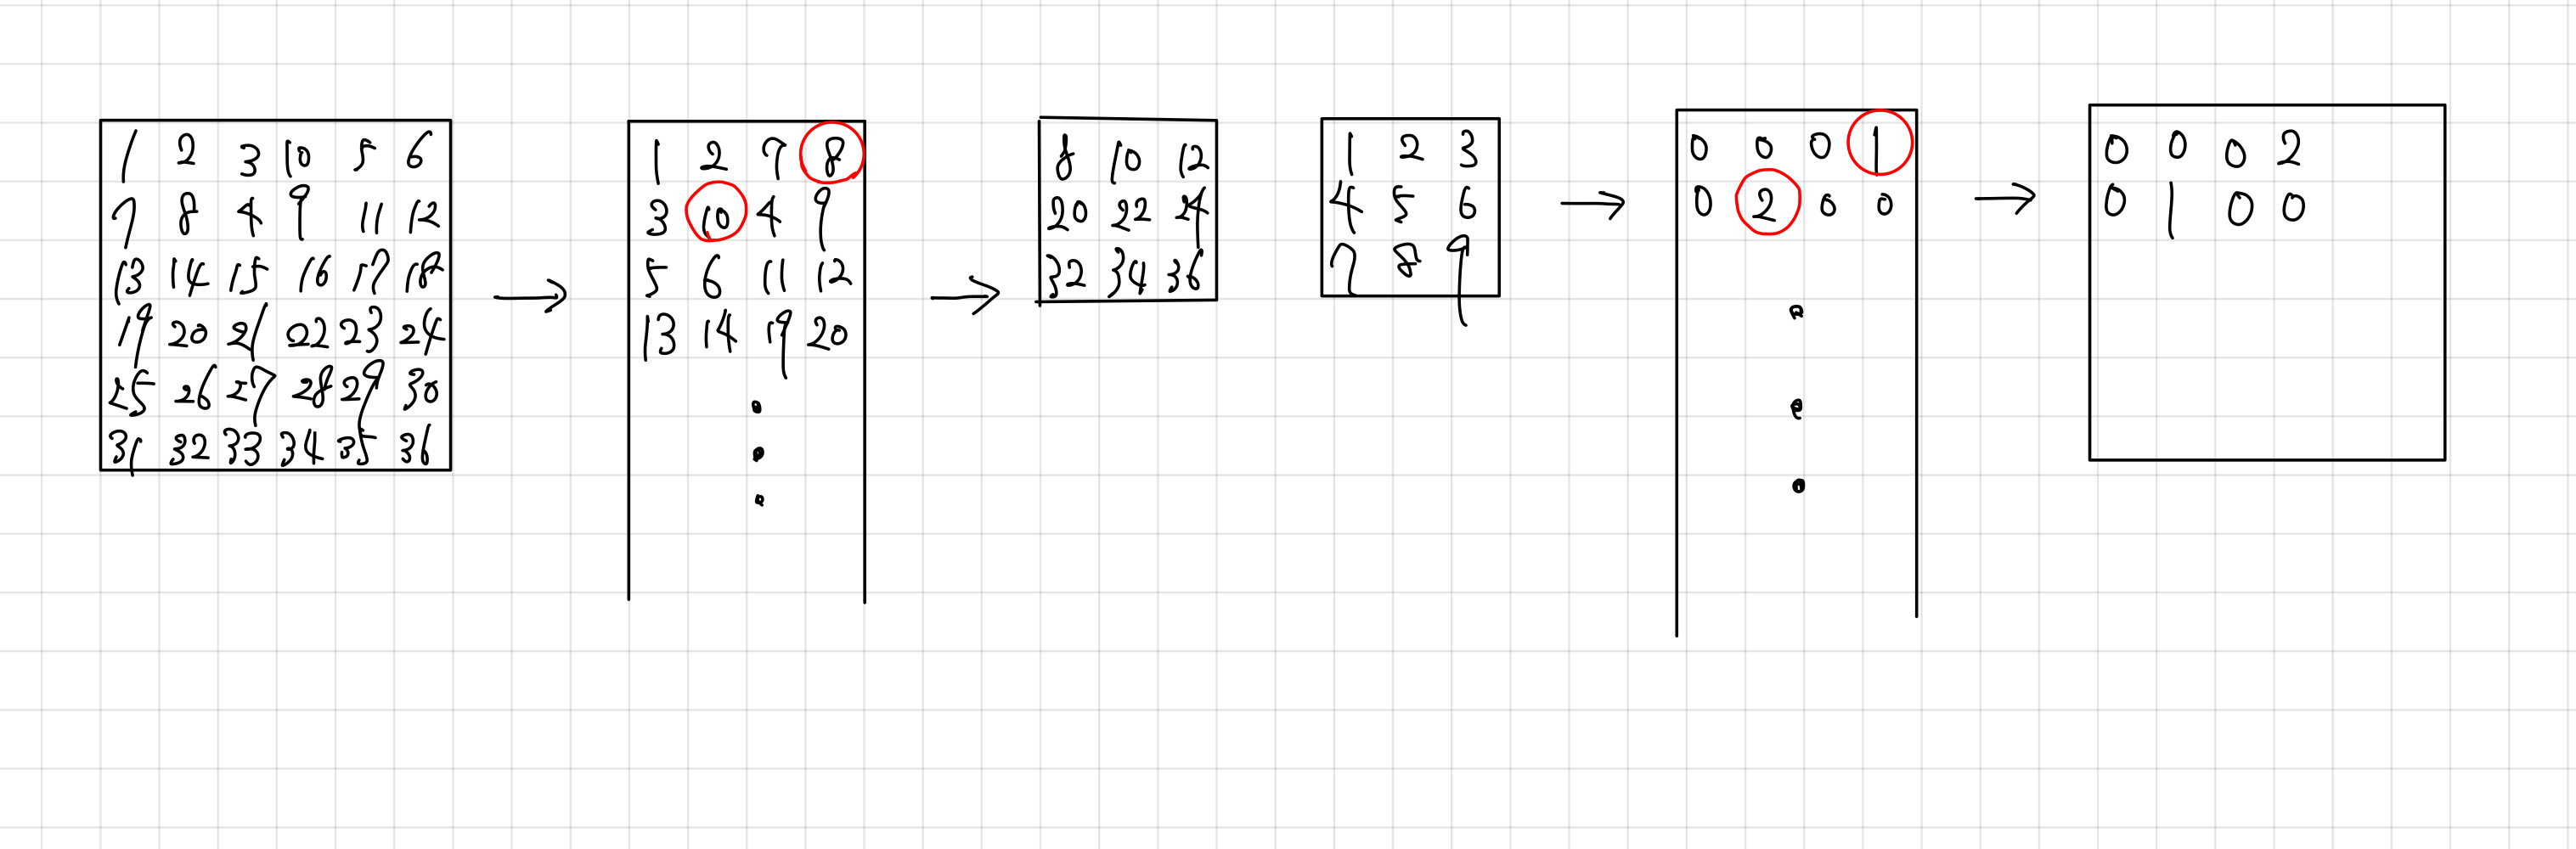
\includegraphics[height = 5cm]{pooling.jpg}
  \caption{pooling}
\end{figure}
まずストライドつきのx2Xを行っている.その後argmaxによって, 最大値を取得する位置を取得している.
これは逆伝播の際に必要になる. そして最大値を取得して, 適切な形に変形すれば, 順伝播は終了である.
次に逆伝播であるが, これはdeltaの形が小さくなったもので得られることに注意し, 0で初期化したものに,
最大値の位置にdeltaを平坦にしたものを代入すればよい. そしてストライド付きのX2xで適切な形に変形すればよい.

実際の実装は以下のとおりである.
\begin{lstlisting}[caption=pooling\_x2X]
  def x2X(self, x):
    w = self.w
    bigL = self.iml - w + 1
    bigW = self.imw - w + 1
    arrayX = np.zeros((self.B, self.ch, w, w, self.outl, self.outw))
    for i in range(w):
        for j in range(w):
            arrayX[:, :, i, j, :, :] = x[:, :, i:i+bigL:w, j:j+bigW:w]
    X = arrayX.transpose(0, 1, 4, 5, 2, 3).reshape(-1, w*w)
    return X
\end{lstlisting}
ストライドが追加されていることに注意したい. ストライド幅はプーリングウィンドウサイズに等しい.

\begin{lstlisting}[caption=pooling\_prop]
  def pooling(self, x, w):
    self.w = w
    self.B, self.ch, self.iml, self.imw = x.shape
    self.outl = self.iml // w
    self.outw = self.imw // w
    X = self.x2X(x)
    self.arg_max = np.argmax(X, axis = 1)
    output1 = np.max(X, axis=1).reshape(
        self.B, self.ch, self.outl, self.outw)
    output2 = output1.transpose(1, 0, 2, 3).reshape(self.B, -1, 1)
    return output1
\end{lstlisting}

\begin{lstlisting}[caption=pooling\_X2x]
  def X2x(self, X):
    w = self.w
    bigL = self.iml - w + 1
    bigW = self.imw - w + 1
    x = np.zeros((self.B, self.ch, self.iml, self.imw))
    arX = X.reshape(self.B, self.ch, self.outl, self.outw, w, w).transpose(0, 1, 4, 5, 2, 3)
    for i in range(w):
        for j in range(w):
            x[:, :, i:i+bigL:w, j:j+bigW:w] = arX[:, :, i, j, :, :]
    return x
\end{lstlisting}

\begin{lstlisting}[caption=pooling\_back]
  def back(self, delta):
    #delta ->  B * (ch* imglen) 
    w = self.w
    delta_x = np.zeros((delta.size, w * w))
    delta_x[np.arange(self.arg_max.size), self.arg_max.flatten()] = delta.flatten()
    return self.X2x(delta_x)
\end{lstlisting}

\section{contest・工夫点}
コンテストに挑戦した. その際にどのような拡張をおこない正答率を
高めたかについて説明する.
もっともいいパラメータを得ることができたのは, ./AdavancedA/CNN.py
である.

\subsection{クラス化}
試行錯誤の過程で様々な拡張を採用したり, 取り除いたりする必要があるために,
Layerや後で説明する拡張を行うものを全てクラス化した. このクラス化したものは
./Layer/以下に入っている.

\subsection{利便性の向上}
学習がいまどれほど進んでいるかを\%表示することや,
途中で打ち切った場合にもそのパラメータを保存することによって,
early-stoppingを行うことができるようになった.

\subsection{model}
汎化性能をなるべく高めたモデルにしたい. そこで汎化性能を高めるLayerを
採用したい. 汎化性能を高めると知られているLayerはDropout, BatchNormalization, Convolution
Layerがある. これを考慮した結果次のような構成になった.
\subsubsection*{Convolution + MaxPooling}
畳み込みを行うことによって, chを増やし表現力を増やす, 加えて文字認識において重要である周辺情報
を利用できるようにする. しかし, これを採用することによって, Dense層が一つしか使えなくなるので,
線形分離しか表現できないこととなる. このため, MaxPoolingWindowは4, 7と大きい幅にして情報を制限しないと
うまく分離できなかった. 結果として, 学習速度, 汎化性能を考えたときに ch=32, window=3, poolwindow=7
がちょうどよい結果となった.
\subsubsection*{BatchNormalization}
Convolutionの結果にBatchNormalizationを行うことによって, 学習の収束速度, 過学習が抑えられる効果があるらしい.
今回はあまり効果を感じなかった. 活性化関数としてRELUを用いている.
\subsubsection*{Dropout}
Dropoutによって疑似的にアンサンブル学習が行われ,汎化性能をあげ過学習を抑える効果があると知られているが,
実際過学習を抑える効果があった.
\subsubsection*{Dense}
全結合層, 活性化関数としてSoftMax関数を用いた.
\subsection{Data-argumentation}
機械学習において精度を高めるために,最も重要なのは訓練データを増やすことである.
しかし, 新たにラベル付けを行うのは時間的コストがかかってしまう.
そこで行うのがオーギュメントである. 例えば, 1の画像を多少平行移動させたり回転させたりしても, それは1と
認識してほしい. そこでラベルをそのままに, 画像を変形させてあげることで, 訓練データを増やすことができる.
今回ランダムにオーギュメントを行いたいので, バッチごとに逐次オーギュメントを行う
(オンラインデータオーギュメント)を行うことにした. contestデータを見ながらどのような拡張を
行うかを決めた.
\subsubsection*{Affine変換}
基本的な拡張であるAffine変換である. 同次座標系を用いない疑似的な実装になってしまった.
次の式を見てもらいたい.
$$
  \begin{pmatrix}
    y1 \\
    y2
  \end{pmatrix}
  = \begin{pmatrix}
    a & b \\
    c & d
  \end{pmatrix}
  \begin{pmatrix}
    x1 \\
    x2
  \end{pmatrix}
  + \begin{pmatrix}
    e \\
    f
  \end{pmatrix}
$$
この計算によって, 回転といった変換が可能である. 簡単のために$
  \begin{pmatrix}
    e \\
    f
  \end{pmatrix} = 0$として説明する.
方針としては
変換後の(i, j)画素の位置の変換前の位置を計算する. これは$\begin{pmatrix}
    a & b \\
    c & d
  \end{pmatrix}$の逆行列を計算し両辺に左から
作用させることによって簡単に得ることが出来る.
$$
  \begin{pmatrix}
    a & b \\
    c & d
  \end{pmatrix}^{-1}
  \begin{pmatrix}
    i \\
    j
  \end{pmatrix} = \begin{pmatrix}
    x1 \\
    x2
  \end{pmatrix}
$$
一般に(x1, x2)は実数なので,線形補完によってその画素の値を計算すればよい. これによって(i, j)の
画素の値が計算できた. 回転させたければ, 回転角を$\theta$として,
$\begin{pmatrix}
    a & b \\
    c & d
  \end{pmatrix} =\begin{pmatrix}
    \cos\theta & -\sin\theta \\
    \sin\theta & \cos\theta
  \end{pmatrix}$
とすれば回転が実現できる. 下図はmnistのトレインデータのはじめ4つに対して
それぞれ$\frac{\pi}{3}, \frac{\pi}{2}$回転させたものを並べたものである.

\begin{figure}[H]
  \centering
  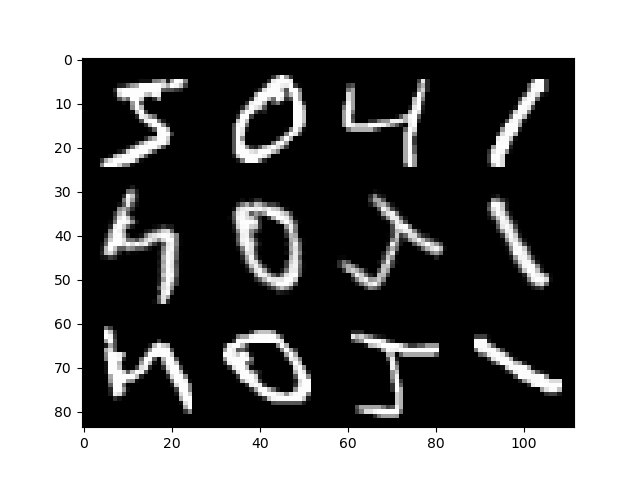
\includegraphics[height = 4cm]{Figure_rotate.png}
  \caption{rotate-image}
\end{figure}

このようにして, スキュー変換, 平行移動, 回転, 拡大に対する頑健性が得られる.
今回のコンテストで最も正答率を高めることができた効果的な拡張であった.
おおよそ8\%の向上がみられた.\footnote{はじめ200個に対してアノテーションを行い, おおよその正答率を計測しています.}

\subsubsection*{gause-noise}
\begin{wrapfigure}{r}[0pt]{0.2\textwidth}
  \centering
  
\includegraphics[width=3cm]{gause-noise.jpg}
  \caption{gause-noise}
  \label{gause}
\end{wrapfigure}

右の図\ref{gause}はコンテストデータの9209番目のデータである.
この画像のようにコンテストデータの中には, 大きくノイズが加わったようなものが見受けられた.
そういったノイズに対する頑健性を得れるように, data-argumentationでも
ノイズを加えるようにする. 今回の実装では, ノイズを平均値1, 分散$\sigma^{2}$
の正規分布から(28, 28)の形で生成し, 元の画像とのアダマール積を出力とした.
このようにすることによって, 1\%ほどの改善が見られた.

\subsubsection*{thickfiltering}
同様にコンテストデータの中には, 文字を太くしたような画像が見られたので,
それに合わせたdata-argumentationを行った. 今回は畳み込みを用いてこれを実装した.
例えば, フィルタを次のようにすると,
$$
  filter =
  \begin{pmatrix}
    0.5 & 0.5 & 0.5 \\
    0.5 & 5   & 0.5 \\
    0.5 & 0.5 & 0.5 \\
  \end{pmatrix}
$$
文字を太くしたような画像が出力される. しかしこのままでは最大値が255を上回ってしまうので,
255以上の値については, 255にするようにしている. 詳しくは図っていないが,
あまり効果は実感できなかった. おそらくConvolution層で行われていることと,
類似性が高いからであると考えた. 以下の図はこのフィルタリングを行った後の, 数字である.
見てわかるように線が太くなっている.
\begin{figure}[H]
  \centering
  \caption{thickfiltering}
  \includegraphics*[width=0.75\linewidth]{thick_filtering.jpg}
\end{figure}

\subsection{正則化}
汎化性能を高める方法として, 正則化が知られている. これは,
パラメーターの自由度を下げることによって, 過学習を防ぎ,
汎化性能を高めるというものである. 実装は非常に簡単であり,
損失関数を以下に変更するだけである. Xを入力, Yを正解ラベル, Wをパラメータとすると,
$$
  L'(X, Y, W) = L(X, Y) + \lambda d(W)
$$
ここでLは通常の損失関数であり, 今回でいうとクロスエントロピーにあたる. そして$\lambda$は正則化項を
どれくらい効かせるかの定数であり, $d$は$W$の重みを表す関数である.
今回はl2正則化を行うこととした. この時, $d(W)$は次のように表せる.
$$
  d(W) = \| W \|_{2}
$$
なので, $w_{ij}$での偏微分式は次のように表せる.
\begin{align*}
  \frac{\partial L'(X, Y, W)}{\partial w_{ij}} & = \frac{\partial L(X, Y)}{\partial w_{ij}} + \lambda \frac{\partial d(W)}{\partial w_{ij}} \\
                                               & = \frac{\partial L(X, Y)}{\partial w_{ij}} + 2\lambda w_{ij}
\end{align*}
つまり, 全体として更新の際に$2\lambda$倍した自分自身を加えれば良いことがわかる.

\subsection{学習方法}
上記のl2正則化を行うと, AdamよりもMomentum付きSGDのほうが性能が良かったので,
学習方法としてはMomentum付きSGDを採用した. 詳しい理由についてはわからなかった.


\subsection{不採用群}
\begin{description}
  \item[optimaizer:SAM] より平坦なところを目指すようにしたoptimizer. 理解も浅いまま実装したが, うまくいかず修正方法も思いつかなったため不採用とした.
    \item[momentumADAM]始めはAdamで学習して, 後半はmomentum付きSGDで学習することによって,
    Adamの学習速度の速さとmomentum付きSGDの汎化性能のいいとこどりを試みたoptimizer.なぜかうまくいかなかった.
    AdamとSGDで収束点が全く違うためと予想している.
  \item[pseudo-labeling] 仮ラベルをつけて学習する. コンテストデータに仮ラベルをつけれればと思ったが
    pseudo-labelingは仮ラベルを正しくつけれないらしい. 実際うまくいかなかった.
  \item[randomcrop] オーギュメントの一種. 画像の一部を切り取る(Dropoutの位置関係つきみたいなことをする).
    おそらく7の横棒を切り取ると1になるが, ラベルは7みたいなことがあるためにうまくいかなかったのではと考察した.
  \item[mixup, cutout] オーギュメント. 上と同じ理由でうまく行かなったと考察した.
  \item[label-smoothing, softlabeling] 6っぽい0と9っぽい0に同じラベル付けをするのは不自然だと考え, 6っぽい0には6の位置にもある程度
    値を与えたものをonehot-vectorとすれば良い(softlabeling).これを実装したかったが,
    もう一つCNNを用意してアンサンブルする以外にsoftlabelingする方法が思いつかなかった. 自分でlabelを付けてしまうと
    それは単に学習を阻害するに終わる. label-smoothingはmnistのlabelは100\%正しくて, 誤ラベルがないためうまくいかなかったと考察した.
\end{description}

\section{問題点A}
正答率が94\%付近で停滞してしまった理由について考える.
今回MaxPoolingのwindowsizeとして7を選択したが,
その場合例えば9をプーリングすると下図5のようになる.
\begin{figure}[h]
  \centering
  
\includegraphics[height = 4cm]{pooling9.jpg}
  \caption{pooling9}
\end{figure}
数字特有の丸が失われてしまう. さらにCovolutionのwindowサイズは3であり, 7より小さいため
この現象を防ぐことはできない. このために例えば9と7の誤認識が非常に
多くなってしまった. これを防ぐためには, poolingwindowサイズを小さくすることが
考えられるが, それでは線形分離が非常に難しくなってしまい, かえって正答率が悪くなってしまった.
これが3層CNNの限界なのではないかと考察する.\footnote{
  kerasで同様の構成を行うと, pool\_size=(2,2)でもうまくいきました.
  その時は96%程度でした. どこかの実装がうまくいってないのかもしれません.
}



\section{B}
自宅デスクトップでの環境構築からGAN作成までの手続きを述べる.
今回自宅デスクトップの利用なのでサーバーでの実行については想定していない.
\subsection{環境}
自分の使っているGPUはNVIDIA GeForce GTX 1650である.
まず, NVIDIAの公式サイトから適切なGPUのドライバの最新をインストールした.
つぎに, VisualStudioをインストールした. この時C++によるデスクトップ開発にチェックを入れなければならないらしい.

次に適切なCUDA, cuDNNをインストールする. おそらく調べたところwindowsは全員GPUによらず, CUDA11.8, cuDNNv8.7.0
でいい? 少なくとも自分は, これでいけました. \footnote{cuDNNのインストールにNVIDIAメンバーシップの会員登録が必要}
cuDNNのファイルをNVIDIA toolkit の適切な場所に配置. (cuDNNのlibの中身はtoolkit/version**/libの中に配置)
pathの設定. サイトによってpathの設定を行ったり, しなかったりとまちまちでしたが, 自分は行いました.
CUDA\_PATH, CUDNN\_PATHをそれぞれNVIDIA GPU toolkit/cuda/v**に指定しました.

anacondanavigatorから新たな仮想環境を追加. root環境でコンフリクトを起こして,
updateもdowngradeも出来ずにanacondaを再インストールする羽目になったため.
その環境にtensorflow-gpuをapplyする. versionは指定した覚えがないが2.6.0が入っていた.
\footnote{うまくいかない場合はterminalでconda update condaとconda update anaconda を行えば自動的にanacondaがversionを調整してくれる
  ようになるらしいです.}

\subsection{環境構築check}
GPUが正しく認識されているかどうかを検査するために以下のコードを実行する.

\begin{lstlisting}[caption=check]
  from tensorflow.python.client import device_lib

    print(device_lib.list_local_devices()) 
\end{lstlisting}
これに対する実行結果は,
\begin{lstlisting}[caption=result\_check]
  GTX 1650, pci bus id: 0000:09:00.0, compute capability: 7.5
  [name: "/device:CPU:0"
  device_type: "CPU"
  memory_limit: 268435456
  locality {
  }
  incarnation: 5875910335587038350
  , name: "/device:GPU:0"
  device_type: "GPU"
  memory_limit: 2240439911
  locality {
    bus_id: 1
    links {
    }
  }
  incarnation: 11886741795246851696
  physical_device_desc: "device: 0, name: NVIDIA GeForce GTX 1650, pci bus id: 0000:09:00.0, compute capability: 7.5"
  ]
\end{lstlisting}

また, もっとも簡単なSequetialモデルによる学習を行うコードは,

\begin{lstlisting}[caption=check2]
  import numpy as np
  import tensorflow.keras as keras
  from tensorflow.keras import datasets, models, layers
  import tensorflow as tf
  import matplotlib.pyplot as plt

  physical_devices = tf.config.list_physical_devices('GPU')
  if len(physical_devices) > 0:
      for device in physical_devices:
          tf.config.experimental.set_memory_growth(device, True)
          print('{} memory growth: {}'.format(device, tf.config.experimental.get_memory_growth(device)))
  else:
      print("Not enough GPU hardware devices available")

  img_rows, img_cols = 28, 28
  num_classes = 10
  (X, Y), (Xtest, Ytest) = keras.datasets.mnist.load_data() 
  X = X.reshape(X.shape[0],img_rows,img_cols,1)
  Xtest = Xtest.reshape(Xtest.shape[0],img_rows,img_cols,1)
  X = X.astype('float32') / 255.0 
  Xtest = Xtest.astype('float32') /255.0
  input_shape = (img_rows, img_cols, 1)
  Y = keras.utils.to_categorical(Y, num_classes) 
  Ytest1 = keras.utils.to_categorical(Ytest, num_classes)


  model = models.Sequential()
  model.add(layers.Conv2D(32, kernel_size=(3,3), activation='relu', input_shape=input_shape, padding='same'))
  model.add(layers.Conv2D(64,(3,3),activation='relu',padding='same'))
  model.add(layers.MaxPooling2D(pool_size=(2,2)))
  model.add(layers.Flatten())
  model.add(layers.Dense(128,activation='relu'))
  model.add(layers.Dense(num_classes, activation='softmax'))
  print (model.summary()) 

  model.compile(
  loss=keras.losses.categorical_crossentropy,
  optimizer=keras.optimizers.SGD(momentum=0.9), metrics=['acc'])

  epochs = 3
  batch_size = 32

  result = model.fit(X,Y, batch_size=batch_size,
  epochs=epochs, validation_data=(Xtest,Ytest1))

  history = result.history

  fig = plt.figure()
  plt.plot(history['loss'], label='loss') 
  plt.plot(history['val_loss'], label='val_loss')
  plt.legend()
  plt.savefig("./AdvanceB/Image/loss_history_withaug.png")
  fig = plt.figure()
  plt.plot(history['acc'], label='acc') 
  plt.plot(history['val_acc'], label='val_acc')
  plt.legend()
  plt.savefig("./AdvanceB/Image/loss_acc_withaug.png") 
\end{lstlisting}

\subsection{B3:GAN}
GANを用いた画像生成器を作れというものが今回の課題の内容である.
GANのアルゴリズムについての説明, 次に実装の方針, 最後に生成された画像とそれに対する考察を行うものとする.

\subsubsection*{GANのアルゴリズム}
GANには大きく分けて二つの構成要素が存在する.
尤もらしい画像を生成する生成器と生成器によって生成された画像か, それともテストデータかを識別する識別機である.
学習の際には, 識別機の学習と, 生成器と識別機を連結させ,識別機のレイヤーをフリーズしたもの(これをGANと呼ぶことにする)の学習を交互に行う.

次により具体的な説明を行う. まず生成器は正規分布から得られた形が(100,)のノイズから最終的に(28, 28)の画像を出力する.
この次元を増やす作業は, Dense層とTransposed Convolution層によって行われる. Transposed Convolution層で行われていることは
単純にはConvolution + MaxPoolingの逆の動作であり, Upsampling + Convolution によって成り立っている.
UpsamplingはMaxPoolingに対応するもので, 例えば(2, 2)を(4, 4)に拡大する. ここでのアルゴリズムは奇数行奇数列
のところにそのまま元の画像を貼り付けて, そして偶数行偶数列のところには左右の値が埋められている所からの線形補間で補われている.
このようにすることによって, 100次元のノイズという圧縮された値から28*28の値へと学習可能なパラメータを用いて拡大することができる.
そして識別機はCNNを用いることができて, 最後のクラス数がC=2であること以外はAdvancedAで実装してきたものとほとんど同じである.

また学習であるが, 識別機の学習は今現在のGeneratorからB/2枚だけ生成させたものと,
Mnist訓練セットからB/2枚だけ取得したものとを連結させたものを1バッチとして, 識別機に入力として与える.
そしてその教師ラベルは$label_x = \begin{cases}
    [0, 1] & (x\in \text{TrainSet})    \\
    [1, 0] & (x\notin \text{TrainSet})
  \end{cases}$として, 次の式を最小化する.
$$
  \underset{\theta_d}{\operatorname{argmin}}\sum_{i=0}^{t}label_{x_i} \cdot \log D(x_i)
$$
ここで$D(X_i)$は識別機の出力である. つまり生成器から出力された画像には $[1, 0]$
に, 訓練データに対しては$[0, 1]$と予測するように学習させる. これは2クラス分類でのクロスエントロピーの最小化と等しい.

次に生成器の学習であるが, 生成器の目的は識別機を騙すことであった.
つまり生成器から出力されたものであるが, 識別機が$[0, 1]$と出力させることが目的である.
そこでGANの入力として(B, 100)のノイズを与えて, 教師ラベルをすべて$[0, 1]$として
同様にバイナリクロスエントロピーを最小化させてあげればよい. ただしこの時, 識別機のパラメータは
更新されないようにする.

しかし, 教科書定義では2クラス分類ではなく識別機の出力を入力データが訓練データに含まれている確率を出力していることに注意したい.
この点で教科書GANの忠実な実装とはなっていない.

\subsubsection*{実装}
実装の方針としては, 次の手順に基づいた.
\begin{enumerate}
  \item generatorモデルの生成. ただし, generator単体で学習させることはないので, コンパイルはする必要はない.
  \item discriminatorモデルの生成. コンパイルまで行う.
  \item discriminatorモデルの全ての層をフリーズさせる. ここでフリーズさせたものを反映させるには
        コンパイルが必要なので, すでにコンパイルを行っている2.で得られたdiscriminatorモデルは依然として学習可能である.
  \item generatorモデルとdiscriminatorモデルを連結してモデル化, その後コンパイルする. これをGANとする.
  \item (discriminatorモデルの事前学習)
  \item discriminatorモデルを1バッチ学習させる.
  \item GANモデルを1バッチ学習させる.
  \item 6. 7. を以降繰り返す.
\end{enumerate}

ここまでは, 比較的簡単に実装できる. GANの特性としてDiscriminatorとgeneratorがが同等程度の賢さでなければならない. 例えば, discriminatorがgenerator
の賢さを大きく上回ってしまうと, generatorは学習ができなくなってしまう. \footnote{実際にその現象は確認できたのですが, discriminatorが賢ければ賢いほどgeneratorの学習が進むような気がします.
  なぜdiscriminatorが強いとダメになってしまうのかがわかりませんでした.}
そのため, 学習率といったハイパーパラメータが非常に重要となる. 次のセクションで自分の調整方法を記す.

\subsubsection*{GANの学習がうまくいかないとき(工夫点)}
GANをg, discriminatorをdと呼ぶことにする.
まず, GANのクロスエントロピーをグラフに出力してみる. その時に滑らかに下がっていることがちょうどいい調整になっている.
クロスエントロピーが著しく上昇していく時は, dが強すぎである. 逆にクロスエントロピーがすぐ下がる一方で, 生成される画像は
望みのものでない場合は, gが強すぎることが考えられる.
ここで自分の場合はdが強くなったので, dを弱くする方法について説明を行う.
\begin{description}
  \item[学習率] Adamの学習率を下げてやればよい. 自分の場合d:3*1e-4, g:1e-4でうまくいった.
  \item[label-smoothing] dの学習の際のラベルを曖昧にする. 例えば, [0, 1]を[0.3, 0.7]にする.
  \item[Dropout] dにDropout層を入れることは, 表現力を落とすことに相当し, 結果的にdを弱くすることができる.
  \item[学習回数] dを一回学習させたあと, gを二回学習させるという繰り返しに変更する.(非推奨らしい)
  \item[BatchNormalization] generatorには畳み込みや全結合層の後ごとにBatchNormalization層を挿入する. dへの挿入は逆効果の場合あり.
\end{description}


\subsubsection*{実行結果}

ある程度数字らしきものが出力されるようになった. 次の画像群はそれぞれ400回, 2000回, 10000回, 50000回繰り返した後の同一乱数から出力された画像である.
\begin{figure}[H]
  \begin{minipage}[b]{0.245\linewidth}
    \centering
    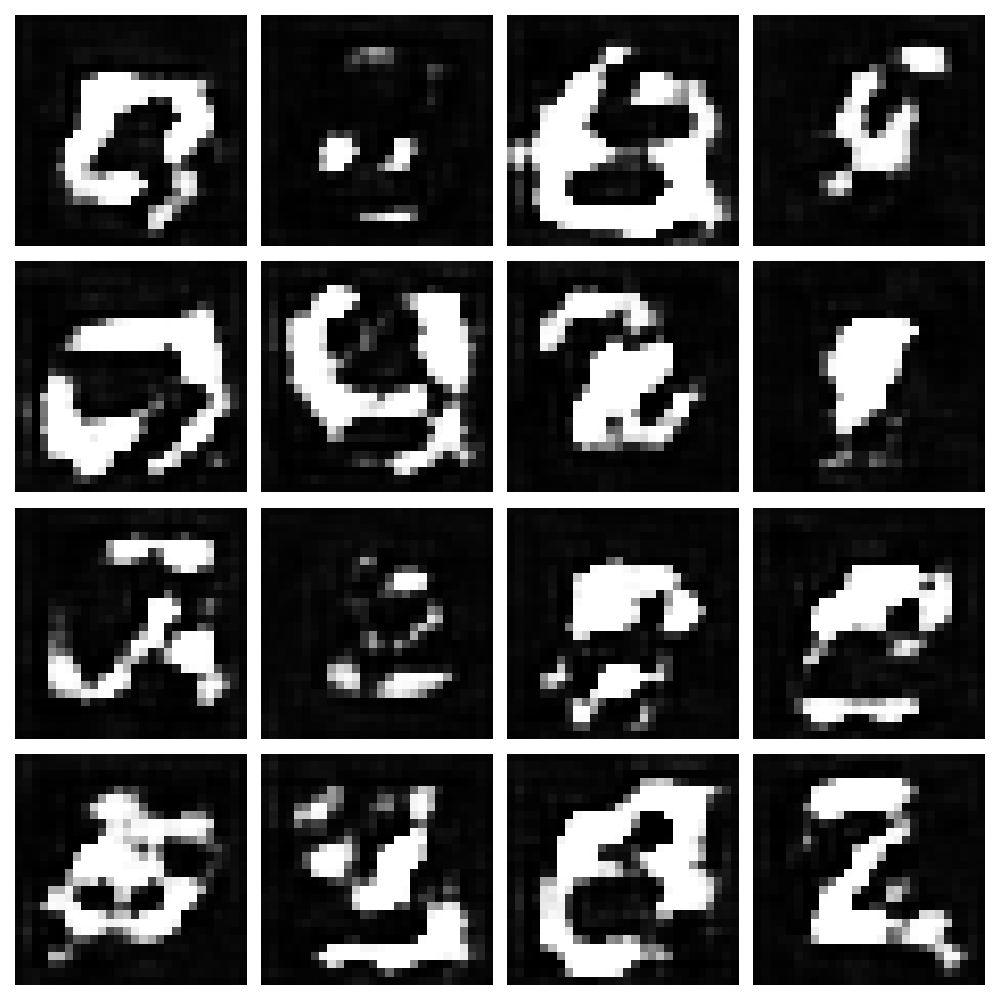
\includegraphics[keepaspectratio, width=0.9\linewidth]{../AdvanceB/Image/result_400.png}
    \caption{GAN:400}
  \end{minipage}
  \begin{minipage}[b]{0.245\linewidth}
    \centering
    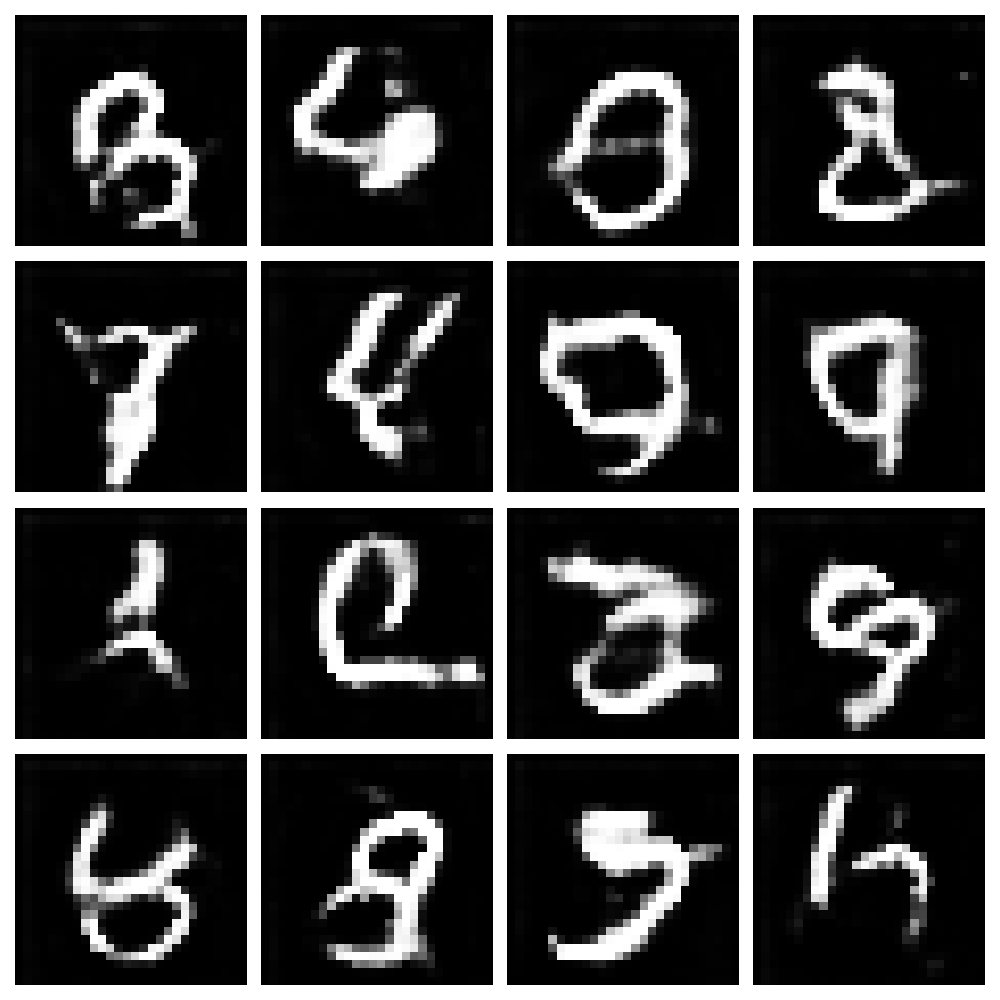
\includegraphics[keepaspectratio, width=0.9\linewidth]{../AdvanceB/Image/result_2000.png}
    \caption{GAN:2000}
  \end{minipage}
  \begin{minipage}[b]{0.245\linewidth}
    \centering
    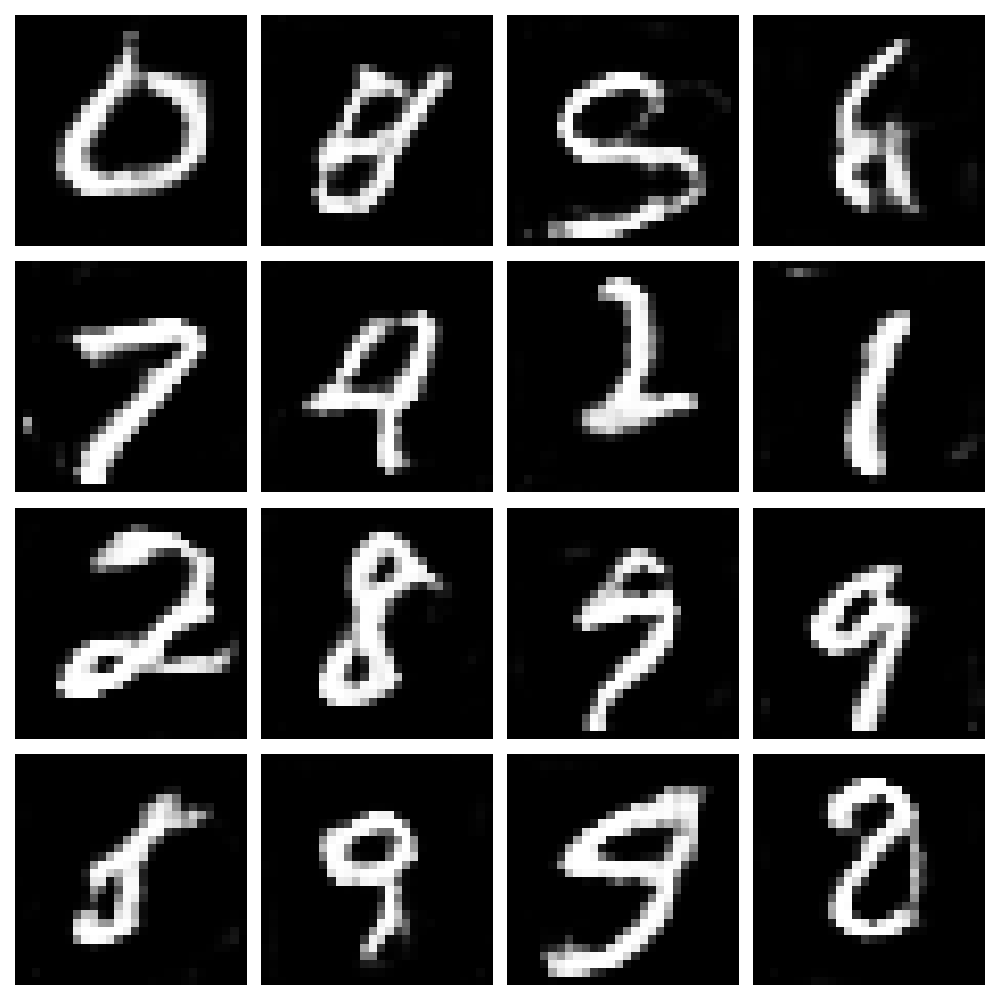
\includegraphics[keepaspectratio, width=0.9\linewidth]{../AdvanceB/Image/result_10400.png}
    \caption{GAN:10000}
  \end{minipage}
  \begin{minipage}[b]{0.245\linewidth}
    \centering
    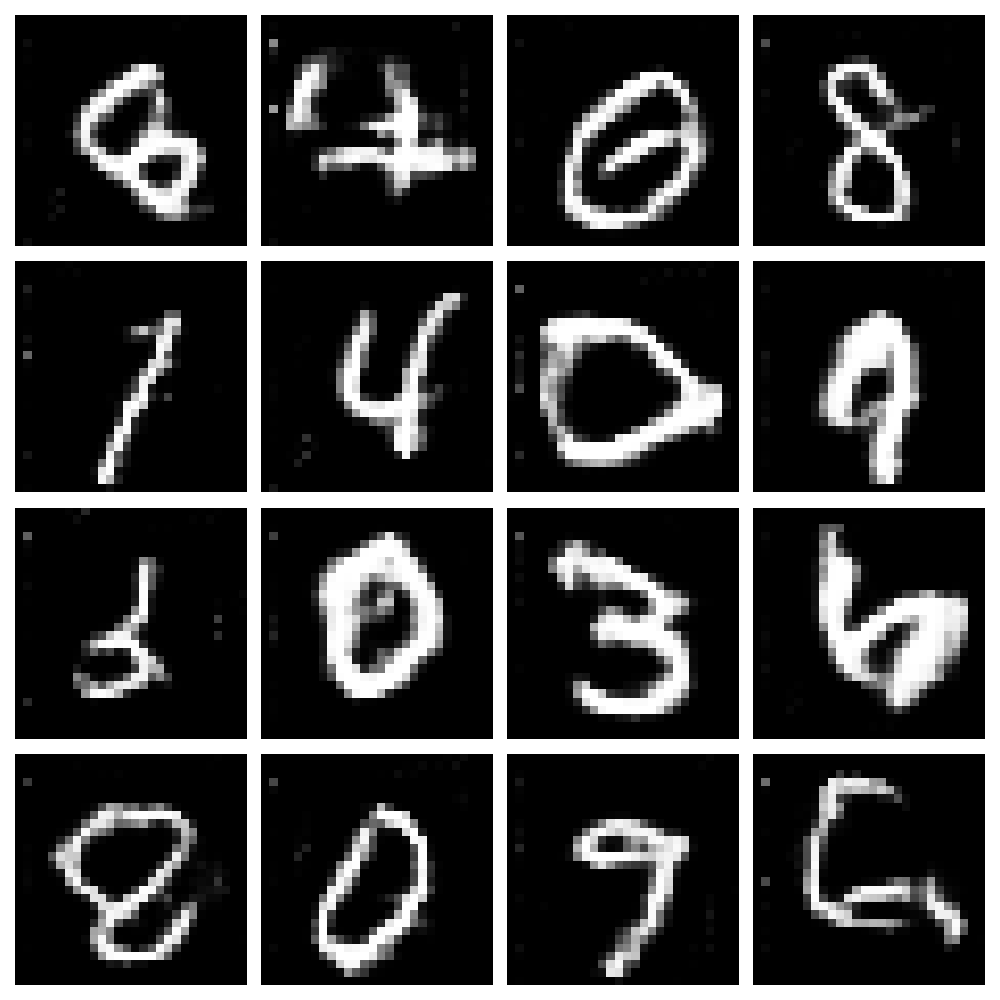
\includegraphics[keepaspectratio, width=0.9\linewidth]{../AdvanceB/Image/result_50000.png}
    \caption{GAN:50000}
  \end{minipage}
\end{figure}

\subsubsection*{問題点B}
generatorのロス的には50000回学習させた地点のほうが低くなっているが,
上の画像を見ると10000回回した所付近が最も自然な文字が出力されていることがわかる.
これを踏まえると, earlystoppingが必要であると考えられるが, この手法を作ることができていない.
そのために, 人力でのearlystoppingが必要となっている.

他にも, ラベルを活かしていないことも挙げられる. 上図を見ればわかるが, 数字らしいものは出力されている一方で
それぞれについて見てみるとどの数字にも分類できないようなものが出力されていることがわかる.
これを防ぐためにmnistの教師labelが有効なのではないかと考えた. もしこのlabelを利用することが出来たならば,
少し発展させれば, 出力される数字の値をランダムではなく, たとえば1のみを生成することも可能になるだろう.
しかしこのラベルの有効な利用には至らなかった.\footnote{Conditional DCGANというものを見つけましたが, 実装には至りませんでした.}



\end{document}